% =========================================================================== %
% Yes. This is a document.

\documentclass[
	english,
	aspectratio=169,
	table
]{beamer}

% =========================================================================== %
% Theme
\usepackage{scrlfile}
	\ReplacePackage{beamerthemeSHUR}{./sty/beamerthemeSHUR}
	\ReplacePackage{beamerinnerthemefancy}{./sty/beamerinnerthemefancy}
	\ReplacePackage{beamerouterthemedecolines}{./sty/beamerouterthemedecolines}
	\ReplacePackage{beamercolorthemechameleon}{./sty/beamercolorthemechameleon}

\usetheme[
	pageofpages=von,
	bullet=circle,
	titleline=true,
	alternativetitlepage=true,
	watermark="",
	watermarkheight=0px,
	watermarkheightmult=0
	]
{SHUR}

% =========================================================================== %
% the usual stuff

\usepackage[utf8]{inputenc}
\usepackage[T1]{fontenc}
\usepackage{babel}
\usepackage{lmodern}
\usepackage{microtype}
\usepackage{csquotes}

\usepackage{tabularx}
\usepackage{booktabs}
\usepackage{multirow}

\usepackage{color, colortbl}
\usepackage{xcolor}
	\definecolor{tabhighlight}{RGB}{230,240,255}

\usepackage{tabto}

\usepackage{minted}
	\usemintedstyle{friendly}

\usepackage{tikz}
	\usetikzlibrary{positioning}
	\usetikzlibrary{matrix}
	\usetikzlibrary{shapes.geometric}
	\usetikzlibrary{backgrounds}
	\usetikzlibrary{calc}
	\usetikzlibrary{decorations.pathreplacing}
	\tikzstyle{every picture}+=[remember picture] 
\usepackage{adjustbox}

\usepackage[most]{tcolorbox}
	\tcbsetforeverylayer
		{colback=cyan!10!white,
		 colframe=cyan!75!black,
		 arc=0pt,
		 outer arc=0pt,
		 parbox=false
		}
	\newtcolorbox{codebox}[1][Code]
		{colback=black!5!white,
		 colframe=blue!40!black,
		 title=#1,
		 leftupper=6mm
		}
	\newtcolorbox{cmdbox}[1][Kommandozeilen-Befehl]
		{colback=black,
		 coltext=white,
		 fontupper=\ttfamily ,
		 colframe=blue!40!black,
		 title=#1,
		 outer arc=0pt
		}
	\newtcolorbox{warnbox}[1][Beachte]
		{colback=black!5!white,
		 colframe=red!40!black,
		 title=#1
		}
	\newtcolorbox{hintbox}[1][Tipp]
		{colback=black!5!white,
		 colframe=green!40!black,
		 title=#1
		}
	\newenvironment{itembox}
		{\begin{tcolorbox}\begin{itemize}}%
		{\end{itemize}\end{tcolorbox}}
	\newtcolorbox{doublebox}[1][.3]
		{righthand width=#1\linewidth,
		 sidebyside,
		 sidebyside gap=6mm,
		 sidebyside align=center,
		 lower separated=false}
	
%==============================================================================%
% GLOBAL MACROS

\newcommand*{\eg}{e.\,g. }
\newcommand*{\ie}{i.\,e. }

\newcommand{\Thus}{\ensuremath{\Rightarrow}}
\newcommand{\thus}{\ensuremath{\rightarrow}}

\newcommand*{\tabcrlf}{\\ \midrule}			% actually still allows for optional argument

\newcommand*{\inPy}[1]{\mintinline{python}{#1}}

% =========================================================================== %

\author{Stefan Hartinger}
\title{Programming in Python}
\subtitle{Part 5: \texttt{while}-Loops and Functions}
\institute{University Regensburg, Department of Theoretical Physics}
\date{Block Course, Summer Term 2021}

% =========================================================================== %

\begin{document}
% =========================================================================== %

\begin{frame}[t,plain]
\titlepage
\end{frame}

% =========================================================================== %

\begin{frame}{Recap}
%
\begin{columns}[T]
\column{.5\linewidth}
\begin{itemize}
\item Modules
	\begin{itemize}
	\item Load with \inPy{import modulename}
	\item Use objects with \inPy{modulename.symbol}
	\end{itemize}
\item \inPy{list}s
	\begin{itemize}
	\item Data containers
	\item Elements in [brackets, separated by commas]
	\item Access with [index in brackets]
	\item Negative indices: count from end, backwards
	\end{itemize}
\end{itemize}
%
\column{.5\linewidth}
\begin{itemize}
\item Slices
	\begin{itemize}
	\item \emph{Extended index}
	\item Creates new (temporary) \inPy{list}
	\item \hspace{0pt} [start : stop : stride]
	\item any of these parameters can be omitted
	\end{itemize}
\item References and copies
	\begin{itemize}
	\item Assignment via \texttt{=} actually assigns references
	\item Module copy
	\item \inPy{copy.deepcopy} for sublists
	\end{itemize}
\item mutable / immutable objects
\end{itemize}

\end{columns}
%
\begin{center}
	\emph{Any Questions?}
\end{center}
%
\end{frame}

% =========================================================================== %

\begin{frame}{Recap}
%
\begin{columns}[T]
\column{.5\linewidth}
\begin{itemize}
\item More containers
	\begin{itemize}
	\item \inPy{str}ings, \inPy{tuple}s, \inPy{set}s und \inPy{dict}s
	\item (im)mutability, uniqueness, keys
	\item \inPy{range}s -- counters
	\end{itemize}
\item \inPy{for}-loops
	\begin{itemize}
	\item \enquote{for each element in container, do ...}
	\item Can be nested
	\end{itemize}
\end{itemize}
%
\column{.5\linewidth}
\begin{itemize}
\item List Comprehension
	\begin{itemize}
	\item Create \inPy{list}s, \inPy{set}s or \inPy{dict}s quickly from \inPy{for}-loops
	\end{itemize}
\item \inPy{enumerate}: generate \inPy{tuple}s of index and container elements
\item \inPy{zip}: combine elements from multiple containers into \inPy{tuple}s
\end{itemize}

\end{columns}
%
\begin{center}
	\emph{Any Questions?}
\end{center}
%
\end{frame}

% =========================================================================== %

\begin{frame}[fragile]
%
\begin{tcbraster}[raster columns=2,
                  raster equal height,
                  nobeforeafter,
                  raster column skip=0.5cm]
\begin{codebox}[Example: Christmas{,} three loops]
\begin{minted}[fontsize=\scriptsize, linenos]{python}
height = 7

for row in range(height) :
  for column in range(height - row) :
    print(" ", end="")
  for column in range(2 * row + 1)  :
    print("*", end="")
  
  print("")
\end{minted}
\end{codebox}
%
\begin{codebox}[Example: Christmas{,} two loops]
\begin{minted}[fontsize=\scriptsize, linenos]{python}
height = 7

for   row    in range(    height    ) :
  for column in range(2 * height + 1) :
    f = abs(column - height) < (row + 1)
    
    print("*" if f else " ", end="")
  print("")
\end{minted}
\end{codebox}
\end{tcbraster}
%
\begin{codebox}[Example: Christmas{,} one loop]
\begin{minted}[fontsize=\scriptsize, linenos]{python}
height = 7

for row in range(height) :
  print(" " * (height - row - 1), "*" * (2 * row + 1))
\end{minted}
\end{codebox}
%
\end{frame}

% =========================================================================== %

\begin{frame}[fragile]{How to Code -- Analysis and Synthesis}
%
\begin{itemize}
\item \emph{Create a String-variable. Find out, how often each character occurs within the text.}
\item \emph{each chacaracter} \Thus Find out, which characters occur at all
	\begin{itemize}
	\item Input: string.
	\item Desired output: list of characters
	\item List \Thus Regard known container types \Thus \inPy{set}: only \emph{unique} elements
	\item Can be formed directly from \inPy{str}ings
	\item[\Thus] Problem partially solved!
	\end{itemize}
\item \emph{how often do they occur in the text} \Thus Count characters
	\begin{itemize}
	\item Input: string, and list (set) of characters
	\item Desired output: list, assignment character $\leftrightarrow$ number
	\item[\Thus] \inPy{dict}
	\item How to count: manually with \inPy{for}-loop
	\item Or automatically: method \inPy{str.count}
	\end{itemize}
\end{itemize}
%
\end{frame}

% =========================================================================== %

\begin{frame}[fragile]
%
%
\begin{codebox}[Example: Count Characters]
\begin{minted}[fontsize=\scriptsize, linenos]{python}
text = "the quick brown fox jumps over the lazy dog"
uniqueChars = set(text)
sortedChars = sorted(uniqueChars)

# Do it manually
counts = {char : 0 for char in uniqueChars}      # create dict with initial value 0
for char in text :                               # count manually
  counts[char] += 1

# Do it automatically
autoCounts = {char : text.count(char) for char in uniqueChars}


print("Analysis of '" + text + "':")
for char in sortedChars :
  print(char, "occurs", counts[char], "times;",
        "automatic count yields", autoCounts[char], ", too")
\end{minted}
\end{codebox}
%
\end{frame}

% =========================================================================== %

\begin{frame}[fragile]{Chapter 5}
%
\begin{itemize}
\item \inPy{while}-Loops
\item Altering the flux of loops
\item \inPy{else} with \inPy{while} and \inPy{for}
\end{itemize}
%
\end{frame}

% =========================================================================== %

\begin{frame}[fragile]{\inPy{while}-Loops}
%
\begin{columns}[T]
\column{.5\linewidth}
\begin{itemize}
\item Idea: Repeat \texttt{[statements]}, as long as \texttt{[condition]} is satisfied (cf. human language)
\item Check \texttt{[condition]} \emph{before} each repetition
\item Possible to create \emph{infinite loops}
	\begin{itemize}
	\item May be intentionally
	\item Most often by mistake
	\item Stop running code:\\
		\texttt{[CTRL] + C} in terminal
	\end{itemize}
\end{itemize}
%
\column{.5\linewidth}
\begin{codebox}[Syntax: \texttt{while}]
\begin{minted}[fontsize=\scriptsize]{python}
while condition :
    statements
\end{minted}
\end{codebox}
\end{columns}
%
\end{frame}

% =========================================================================== %

\begin{frame}[fragile]
%
\begin{codebox}[Example: Compound Interest (I)]
\begin{minted}[linenos, fontsize=\scriptsize]{python}
capital  = float(input("Please provide your seed capital:"))
interest = float(input("Please provide the interest rate:"))
limit    = float(input("Please provide the savings goal :"))

years    = 0

while capital < limit :
    capital *= 1 + interest
    years   += 1

print("After", years, "years you've reached your savings goal.")
\end{minted}
\end{codebox}
%
\end{frame}
% =========================================================================== %

\begin{frame}[fragile]{Altering the flux of loops: \inPy{break}}
%
\begin{itemize}
\item Loops (\ie both, \inPy{while} and \inPy{for}) can be exited at any time
\item Useful for secondary conditions within the loop
\item Should be coupled to a condition\\
 \Thus \inPy{if}
\item Nested loops: exit \emph{current level}
	\begin{itemize}
	\item If you want to leave \emph{multiple levels}: Use flags
	\end{itemize}
\end{itemize}
%
\end{frame}

% =========================================================================== %

\begin{frame}[fragile]
\begin{codebox}[Beispiel: \texttt{break} with a single level]
\begin{minted}[linenos, fontsize=\scriptsize]{python}
count = 0
value = 0

while count < 12 :
    newValue = float(input("Please provide a value: "))
    value += newValue
    count += 1
  
    if value > 9000 :
        value = "over nine thousand!!"
        break
  
    print("Current total after entering", count, "values:", value)

print("Total:", value)
\end{minted}
\end{codebox}
\end{frame}

% =========================================================================== %

\begin{frame}[fragile]
\begin{codebox}[Example: \texttt{break} with multiple levels]
\begin{minted}[linenos, fontsize=\scriptsize]{python}
import random

total = 0
quitFlag = False

while total < 10 :
    batch = [random.randint(-3, 20) for i in range(5)]
    
    for num in batch :
        print(num, end = ", ")

        if num < 0:
            print("secondary condition: negative number")
            quitFlag = True
            break
            
        if quitFlag : break
        total += num
    
print("total:", total)
\end{minted}
\end{codebox}
\end{frame}

% =========================================================================== %

\begin{frame}[fragile]{Altering The Control Fulx: \inPy{continue}}
%
\begin{itemize}
\item Skip rest of loop body \emph{without exiting it}
\item Works for both, \inPy{while} and \inPy{for}
\item Usually with \Thus \inPy{if}, too
\end{itemize}
%
\begin{codebox}[Example: \texttt{continue}]
\begin{minted}[linenos, fontsize=\scriptsize]{python}
container = []
while len(container) < 3 :
    value = int(input("Please provide an even number: "))
    
    if value % 2 :
        print(value, "is odd and hence invalid.")
        continue
        
    container.append(value)
    print("Input so far: ", container)

print("done.")
\end{minted}
\end{codebox}
%
\end{frame}

% =========================================================================== %

\begin{frame}[fragile]{\inPy{else} with \inPy{while} and \inPy{for}}
%
\begin{itemize}
\item Idea \enquote{if not applicable}
\item \inPy{else}-block is executed, if a loop terminates \emph{regularly}, \ie if it is not exited via \inPy{break}
\item For both, \inPy{for} and \inPy{while}
\end{itemize}
%
\end{frame}

% =========================================================================== %

\begin{frame}[fragile]
%
\begin{codebox}[Example: Compound Interest (II)]
\begin{minted}[linenos, fontsize=\scriptsize]{python}
capital  = float(input("Please provide your seed capital:"))
interest = float(input("Please provide the interest rate:"))
limit    = float(input("Please provide the savings goal :"))

years    = 0
while capital < limit :
    capital *= 1 + interest
    years   += 1
    
    if capital < limit :
        break
else :
    print("Your seed capital is already big enough.")
  
print("After", years, "years you've reached your savings goal.")
\end{minted}
\end{codebox}
%
\end{frame}

% =========================================================================== %

\begin{frame}[fragile]
%
\begin{codebox}[Example: \texttt{for} with \texttt{break}{,} \texttt{continue} and \texttt{else}]
\begin{minted}[linenos, fontsize=\scriptsize]{python}
tasks = [("hidden", "watch Fullmetal Alchemist"),
         ("open", "work very hard on Python"),
         ("open", "drink all the coffee")]
         
search = ["watch", "work"]

for keyword in search :
    for ID, (state, task) in enumerate(tasks) :
        if state == "hidden" : continue
        if keyword in task :
            print(keyword, "was found in task ID", ID)
            break
    else :
        print(keyword, "was not found in the tasks.")
\end{minted}
\end{codebox}
%
\begin{cmdbox}[Output: \texttt{for} with \texttt{break}{,} \texttt{continue} and \texttt{else}]
\begin{minted}[fontsize=\scriptsize]{text}
watch was not found in the tasks.
work was found in task ID 1
\end{minted}
\end{cmdbox}
%
\end{frame}

% =========================================================================== %

\begin{frame}[fragile]{Chapter 6}
%
\begin{itemize}
\item Functions
\item By-Value- and By-Reference-Parameters
\item Scopes
\end{itemize}
%
\end{frame}

% =========================================================================== %

\begin{frame}[fragile]
%
\begin{columns}[T]
\column{.5\linewidth}
\begin{Large}
{Functions}
\vspace{6pt}
\end{Large}
\begin{itemize}
\item Idea: Combine multiple, recurring steps into a single command
\item Can be parametrised (Example: Output of text in a box)
\item Can return a result (\Thus \emph{function} in its mathematical sense)
\item \inPy{return}: exit function, return to where it was called
\inPy{return result}: same as above, plus: \enquote{report} a result
\item Without \inPy{return}: jump-back automatically after last command
\item Implicit return value \inPy{None}
\end{itemize}
%
\column{.5\linewidth}
\begin{codebox}[Syntax: Definition of Functions]
\begin{minted}[fontsize=\scriptsize]{python}
def functionName (parameters) :
    statements
    return result
\end{minted}
\end{codebox}
%
\begin{codebox}[Syntax: Calling a Function]
\begin{minted}[fontsize=\scriptsize]{python}
functionName(parameters)
variable = functionName(parameterlist)
\end{minted}
\end{codebox}
%
\begin{hintbox}[Order of Code]
Funktions have to be defined \emph{before} they are called for the first time.
\end{hintbox}
\end{columns}
%
\end{frame}

% =========================================================================== %

\begin{frame}[fragile]{Parameters (aka Arguments)}
%
\begin{itemize}
\item Function oversees \emph{its own set of new variables}. Initial values as \enquote{sent} at the call
\item In definition: variable names, separated by commas
\item In call: expressions, separated by commas
\item Thought model: Working copy of the \emph{evaluated} expressions is stored in \emph{local} variables of the functions
\end{itemize}
%
\begin{tcbraster}[raster columns=2,
                  raster equal height,
                  nobeforeafter,
                  raster column skip=0.5cm]
\begin{codebox}[Example: Evolution of Values]
\begin{minted}[fontsize=\scriptsize, linenos]{python}
def func(x, y) :
   print(x, y)
   x, y = 5, 5
   print(x, y)

x = 3
func(x, x + 5)
print(x)   
\end{minted}
\end{codebox}
%
\begin{tcolorbox}[title=Evolution of Values]
\scriptsize
\begin{center}
\begin{tabular}{l|ccc}
Line & $x_{main}$ & $x_{func}$ & $y_{func}$ \tabcrlf
6 & 3 & -- & -- \\
2 & 3 &  3 &  8 \\
3 & 3 &  5 &  5 \\
4 & 3 &  5 &  5 \\
8 & 3 & -- & --
\end{tabular}
\end{center}
\end{tcolorbox}
\end{tcbraster}
%
\end{frame}

% =========================================================================== %

\begin{frame}[fragile]
%
\begin{codebox}[Example: Exponential as a Funktion]
\begin{minted}[linenos, fontsize=\scriptsize]{python}
def expFunction(x0) :
    x           = 1.0
    denominator = 1.0
    result      = 1.0
    iterations  = 10
    for k in range(1, iterations) :
        x            *= x0
        denominator  *= k
        result += x / denominator
    return result

EulersNumber = expFunction(1.0)             # Call function, store result in variable
print(f"Euler's Number is {EulersNumber}")
print(f"e³ = {expFunction(3.0)}")           # Forward result to another function
\end{minted}
\end{codebox}

\begin{cmdbox}[Output: Exponential as a Funktion]
\begin{minted}[fontsize=\scriptsize]{text}
Euler's Number is 2.7182815255731922
e³ = 20.063392857142855
\end{minted}
\end{cmdbox}
%
\end{frame}

% =========================================================================== %

\begin{frame}[fragile]
%
\begin{codebox}[Example: Funktion \enquote{without} Return Value]
\begin{minted}[linenos, fontsize=\scriptsize]{python}
import math

def printBoxed(text, boxSize) :
    lenText     = len(text)
    countSpaces = boxSize - lenText - 2        # 2 spaces for |borders|
    spacesLeft  = math.floor(countSpaces / 2)  # round down
    spacesRight = math.ceil (countSpaces / 2)  # round up
    print("+" +               (boxSize - 2) * "-"           + "+")
    print("|" + spacesLeft * " " + text + spacesRight * " " + "|")
    print("+" +               (boxSize - 2) * "-"           + "+")
reVal = printBoxed("Don't forget to be awesome!", 60)
print("The function returned:" , reVal)
\end{minted}
\end{codebox}

\begin{cmdbox}[Output: Funktion \enquote{without} Return Value]
\begin{minted}[fontsize=\scriptsize]{text}
+----------------------------------------------------------+
|               Don't forget to be awesome!                |
+----------------------------------------------------------+
The function returned: None
\end{minted}
\end{cmdbox}
%
\end{frame}

% =========================================================================== %

\begin{frame}[fragile]{By-Value und By-Reference-Parameter}
%
\begin{itemize}
\item Function \enquote{doesn't know}, where original information was stored (\emph{no} pass by reference)
\item Picture: Pass on a working copy (pass by value) -- only partially correct
\item In fact: working copy of \emph{addresses}
\end{itemize}
%
\begin{tcbraster}[raster columns=2,
                  raster equal height,
                  nobeforeafter,
                  raster column skip=0.5cm]
\begin{codebox}[Example: Passing a referenz by value]
\begin{minted}[fontsize=\scriptsize, linenos]{python}
def foobar(data) :
    data.append(1)
    data = data + [2]
    print("in foobar: data =", data)
data = []
foobar(data)
print("on module level: data =", data)
\end{minted}
\end{codebox}
%
\begin{cmdbox}[Output: Passing a referenz by value]
\begin{minted}[fontsize=\scriptsize]{text}
in foobar: data = [1, 2]
on module level: data = [1]
\end{minted}
\end{cmdbox}
\end{tcbraster}
%
\end{frame}

% =========================================================================== %

\begin{frame}[fragile]
%
\begin{tcolorbox}[title=Memory Model]
\begin{center}
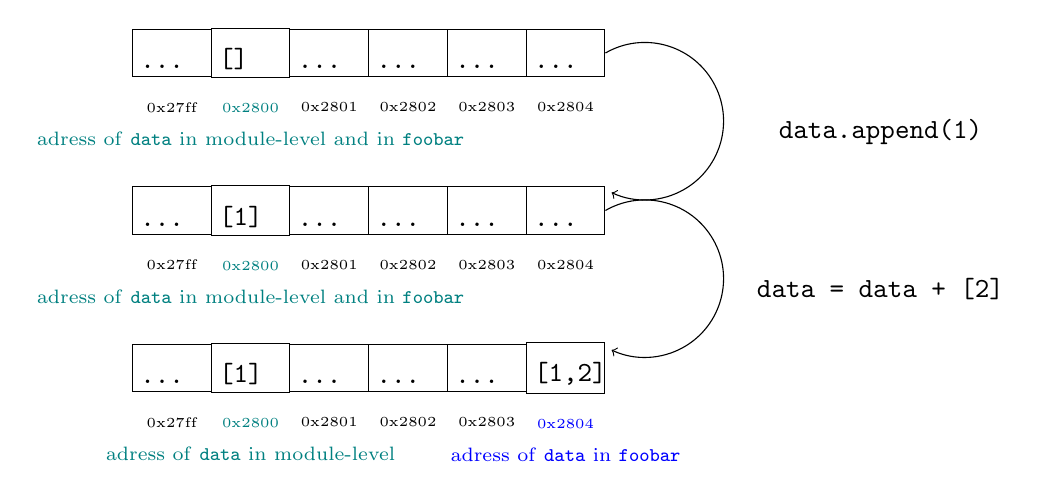
\begin{tikzpicture}
  [ 
    cell/.style={text width=8mm,
      text height=4mm, draw=black, inner sep=1mm},
    ld/.style={draw=blue,shorten >=2pt,->}
  ]
  \node (a1) at (0,4) [cell] {\ttfamily ...};
  \node (a2) at (1,4) [cell] {\ttfamily  []};
  \node (a3) at (2,4) [cell] {\ttfamily ...};
  \node (a4) at (3,4) [cell] {\ttfamily ...};
  \node (a5) at (4,4) [cell] {\ttfamily ...};
  \node (a6) at (5,4) [cell] {\ttfamily ...};

  \node (b1) at (0,2) [cell] {\ttfamily ...};
  \node (b2) at (1,2) [cell] {\ttfamily [1]};
  \node (b3) at (2,2) [cell] {\ttfamily ...};
  \node (b4) at (3,2) [cell] {\ttfamily ...};
  \node (b5) at (4,2) [cell] {\ttfamily ...};
  \node (b6) at (5,2) [cell] {\ttfamily ...};

  \node (c1) at (0,0) [cell] {\ttfamily ...};
  \node (c2) at (1,0) [cell] {\ttfamily [1]};
  \node (c3) at (2,0) [cell] {\ttfamily ...};
  \node (c4) at (3,0) [cell] {\ttfamily ...};
  \node (c5) at (4,0) [cell] {\ttfamily ...};
  \node (c6) at (5,0) [cell] {\ttfamily [1,2]};
  
  \node (A1) [below=2mm of a1]             {\tiny 0x27ff};
  \node (A2) [below=2mm of a2, color=teal] {\tiny 0x2800};
  \node (A3) [below=2mm of a3]             {\tiny 0x2801};
  \node (A4) [below=2mm of a4]             {\tiny 0x2802};
  \node (A5) [below=2mm of a5]             {\tiny 0x2803};
  \node (A6) [below=2mm of a6]             {\tiny 0x2804};
  
  \node (B1) [below=2mm of b1]             {\tiny 0x27ff};
  \node (B2) [below=2mm of b2, color=teal] {\tiny 0x2800};
  \node (B3) [below=2mm of b3]             {\tiny 0x2801};
  \node (B4) [below=2mm of b4]             {\tiny 0x2802};
  \node (B5) [below=2mm of b5]             {\tiny 0x2803};
  \node (B6) [below=2mm of b6]             {\tiny 0x2804};
  
  \node (C1) [below=2mm of c1]             {\tiny 0x27ff};
  \node (C2) [below=2mm of c2, color=teal] {\tiny 0x2800};
  \node (C3) [below=2mm of c3]             {\tiny 0x2801};
  \node (C4) [below=2mm of c4]             {\tiny 0x2802};
  \node (C5) [below=2mm of c5]             {\tiny 0x2803};
  \node (C6) [below=2mm of c6, color=blue] {\tiny 0x2804};



  \node (main1) [below=0mm of A2, color=teal] {\scriptsize adress of \texttt{data} in module-level and in \texttt{foobar}};
  \node (main2) [below=0mm of B2, color=teal] {\scriptsize adress of \texttt{data} in module-level and in \texttt{foobar}};
  \node (main3) [below=0mm of C2, color=teal] {\scriptsize adress of \texttt{data} in module-level};
  \node (func)  [below=0mm of C6, color=blue] {\scriptsize adress of \texttt{data} in \texttt{foobar}};
  
  \draw [->] (a6.east)arc(120:-115:1.0);		%start angle: stop angle : radius  
  \node (step1) at (9,3) {\texttt{data.append(1)}};
  \draw [->] (b6.east)arc(120:-115:1.0);
  \node (step1) at (9,1) {\texttt{data = data + [2]}};
\end{tikzpicture}
\end{center}
\end{tcolorbox}
%
\end{frame}

% =========================================================================== %

\begin{frame}[fragile]
%
\begin{codebox}[Example: Passing Immutables]
\begin{minted}[linenos, fontsize=\scriptsize]{python}
def foobar(data) :
    data = 2
    print("in foobar: data =", data)

data = 1
foobar(data)
print("on module level: data =", data)
\end{minted}
\end{codebox}

\begin{cmdbox}[Output: Passing Immutables]
\begin{minted}[fontsize=\scriptsize]{text}
in foobar: data = 2
on module level: data = 1
\end{minted}
\end{cmdbox}
%
\end{frame}

% =========================================================================== %

\begin{frame}{Scopes}
%
\begin{itemize}
\item Code in function is \emph{separate} from the rest of the code
\item Variables in a functions only exist \emph{locally}
\item Lingu: Functions have their own \emph{scope}, variables belong to a scope
\item In a function-scope you can \enquote{see} outside variables, but not vice versa
\item Parameter list: variables of the function scope
\item Local re-definition possible
\item But: not after first read-access
\end{itemize}
%
\end{frame}

% =========================================================================== %

\begin{frame}[fragile]
%
\begin{codebox}[Example: Local Variables]
\begin{minted}[linenos, fontsize=\scriptsize]{python}
globVar  = ["foo"]
reDefVar = ["bar"]

def foobar() :
    locVar = "confused cat"         # local definition
    reDefVar = [42]                 # redefinition -- local variable
    print(globVar, reDefVar)        # globVar: module level; reDefVar: local scope
    globVar.append("foo bar")       # write access; adress doesn't change
    #globVar = globVar + ["baz"]    ! error: would change adress

foobar()

print(globVar, reDefVar)
# print(locVar)                     ! error: 'locVar' is local to foobar
\end{minted}
\end{codebox}
\begin{cmdbox}[Output: Local Variables]
\begin{minted}[fontsize=\scriptsize]{text}
['foo'] [42]
['foo', 'foo bar'] ['bar']
\end{minted}
\end{cmdbox}
%
\end{frame}

% =========================================================================== %

\begin{frame}
%
\begin{hintbox}[KISS: Keep It Simple{,} Stupid]
\emph{KISS} is a design principle in software development: \emph{Keep it simple, stupid}.

Adhering to the idea, I advise you to follow these rules:

\begin{itemize}
\item Only \enquote{way into to function} is the parameter list
\item Only \enquote{way out of the function} is the return value
\item All variables used in a function are defined before reading them, preferrably in the first few lines of the function. Thus, they all are \emph{local variables}.
\end{itemize}

Otherwise, dependencies can become rather complicated, difficult to control and will be sources of errors. You need to be able to controll all data going into and out of your functions; this is hard if you can't see which data do go in. Essentially, you'd need to know the state of your \emph{entire programm, at all times}.
\end{hintbox}
%
\end{frame}
\end{document}

% MAREI!!
% whom do I give credit? Where?